\chapter{Background Estimation and Systematics}

\section{Introduction}

\section{QCD Background}

\section{Electroweak Background}

Electroweak processes can have real MET due to neutrinos which are not
detected by CMS. There are two components to the electroweak background:
$W\rightarrow e\nu$, where the electron is misidentified as a photon and 
$\gamma Z\rightarrow\gamma\nu\nu$, which has a real photon and real MET. \\

The $W\rightarrow e\nu$ background is estimated by measuring the electron/photon
misidentification rate in data. \\

The $\gamma Z\rightarrow\gamma\nu\nu$ background is estimated from Monte Carlo.

\section{Electron/Photon Fake Rate}

Measuring the fraction of electrons that are misidentified as photons is
important for estimating the background coming from $W\rightarrow e\nu$ events
where the electron is misidentified as a photon. \\

With a fake rate, $f_{e\rightarrow\gamma}$, and given a true number of
$Z\rightarrow ee$ events, $N_{Z}$, the number of events in the ee sample is
given by $N_{ee} = (1 - f_{e\rightarrow\gamma})^{2}N_{Z}$. And the number of
events in the e$\gamma$ is given by $N_{e\gamma} = 2[f_{e\rightarrow\gamma}(1 -
f_{e\rightarrow\gamma})]N_{Z}$. With measurements of $N_{ee}$ and $N_{e\gamma}$
the fake rate can be determined as $f_{e\rightarrow\gamma} =
N_{e\gamma}/(2N_{ee} + N_{e\gamma})$. \\

The fake rate is measured using an ee sample and an e$\gamma$ sample from data.
Electrons are selected using the same requirements as photons, but with a pixel
seed required (rather than no pixel seed). The number of $Z\rightarrow ee$
events in each sample is determined by fitting a Crystal Ball function with a
linear background assumption (Figure \ref{fig:Zee_Fit}). There is no significant
difference in the yields if a constsnt or quadratic background shape is used. \\

\begin{figure}
\begin{center}
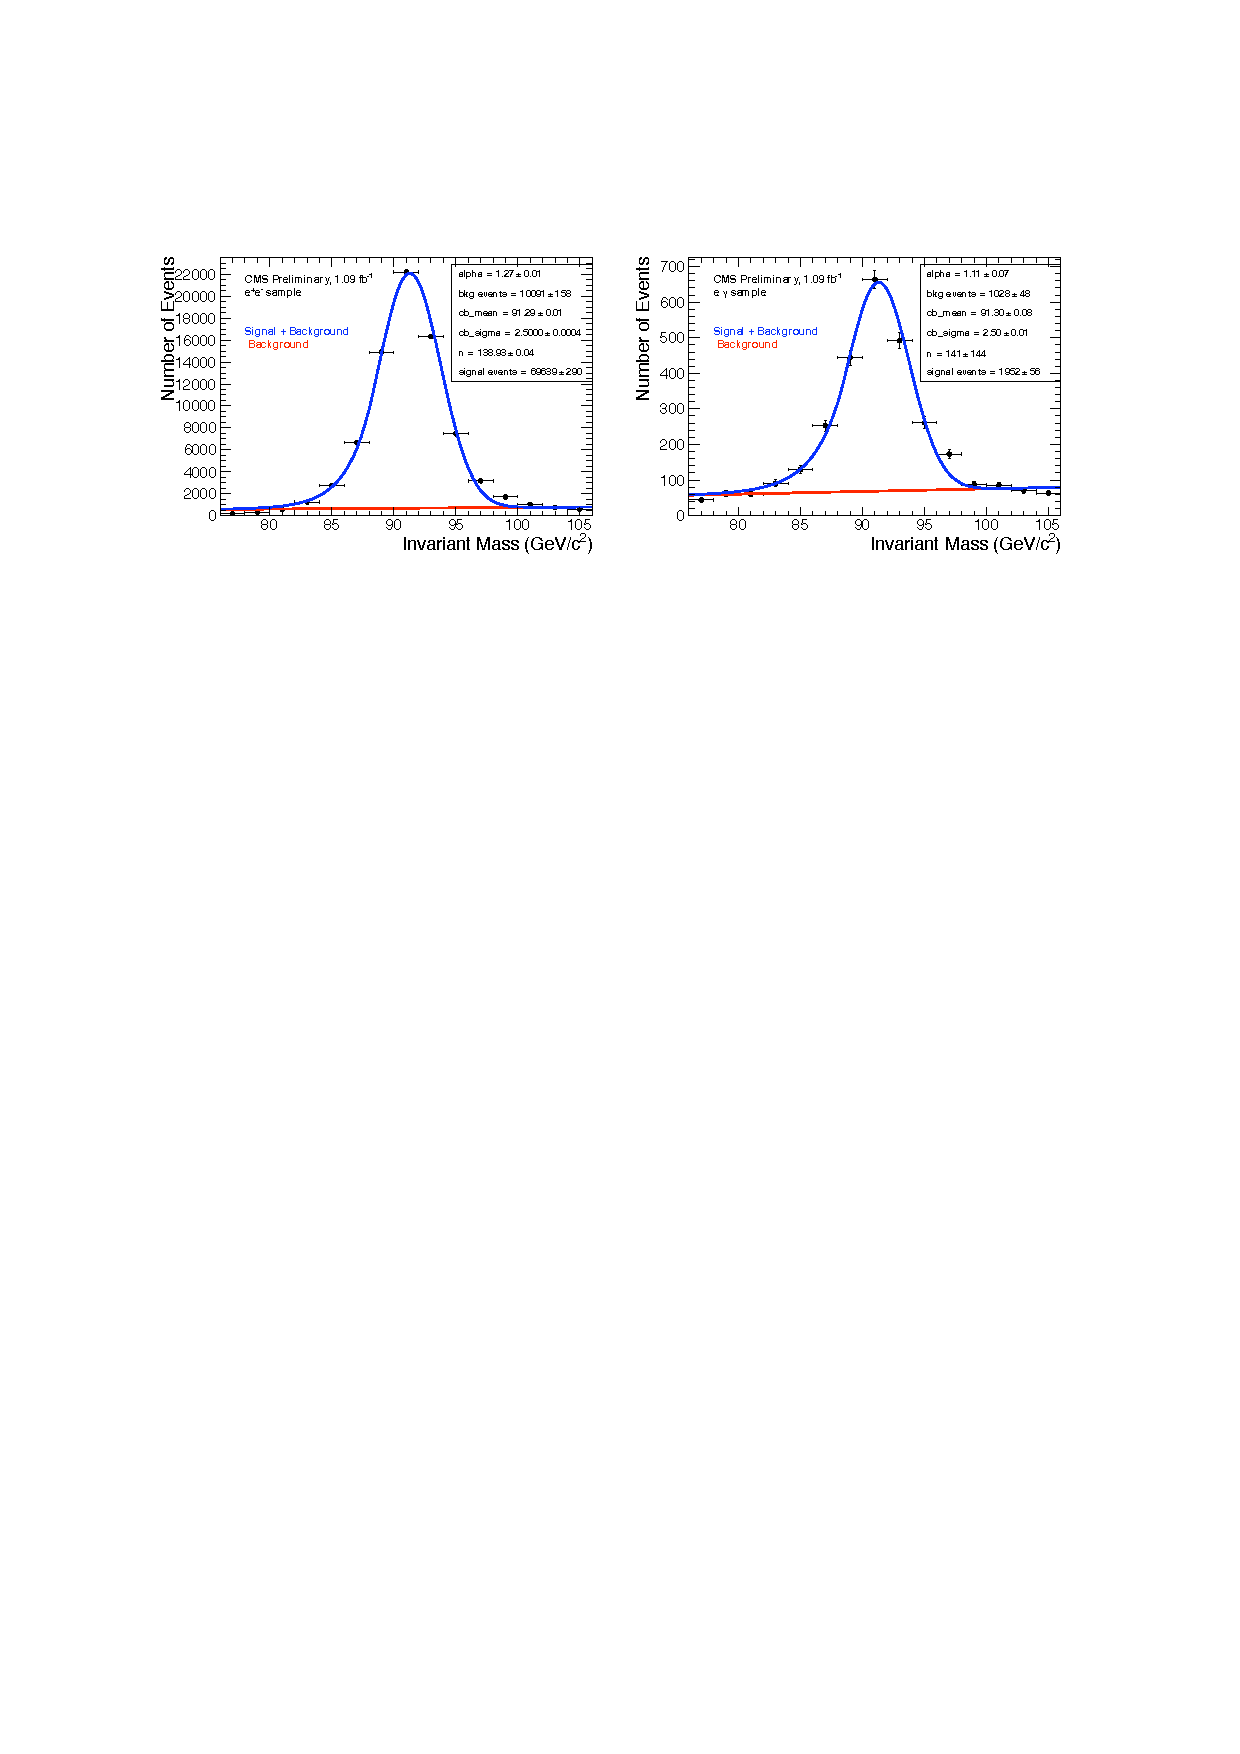
\includegraphics[width=1.0\textwidth]{Zee_Fit.pdf}
\end{center}
\caption{The invariant mass of ee and e$\gamma$ candidates. The Z peak is fitted
using a Crystal Ball function and a linear background.}
\label{fig:Zee_Fit}
\end{figure}

The fit of the Z peak in the ee sample yields $69639 \pm 290$ Z events. Fitting
the Z peak in the e$\gamma$ sample yield $1952\pm56$ Z events. From these
numbers the misidentification rate is $f_{e\rightarrow\gamma} = 0.014\pm0.004$.
This number varies little as a function of e or $\gamma$ $p_{T}$. Based on the
variations with $p_{T}$ a systematic uncertainty of 0.002 is assigned to
$f_{e\rightarrow\gamma}$. 

\section{Photon Efficiency}

The photon efficiency needs to be determined to calculate the signal efficiency.
The photon efficiency could be found using the MC, but that relies heavily on
the correct modelling of the shower shape, isolation and other variables which
may not be well modelled in the MC. The photon efficiency should be measured
from data. In the absence of any pure photon sample in the data, electrons from 
$Z\rightarrow ee$ events are used. This relies on the similarity in detector 
response between electrons and photons. A scale factor to correct the MC photon
efficiency to the real photon efficiency in data is obtained using the
electrons (Equation \ref{eq:Scale_Factor}). \\

\begin{equation}
\epsilon_{\gamma}^{data} = \frac{\epsilon_{e}^{data}}{\epsilon_{\gamma}^{MC}}
\times \epsilon_{\gamma}^{MC}
\label{eq:Scale_Factor}
\end{equation}  

Where:
\begin{itemize}
\item $\epsilon_{\gamma}^{data}$ = photon efficiency in data;
\item $\epsilon_{\gamma}^{MC}$ = photon efficiency in MC;
\item $\epsilon_{e}^{data}$ = electron efficiency obtained using $Z\rightarrow
ee$ events in data that satisfy the photon selection; 
\item $\epsilon_{e}^{MC}$ = electron efficiency obtained using $Z\rightarrow ee$
events in MC that satisfy the photon selection. 
\end{itemize}

The selection critrea for electrons are the same as those for photons except 
that electrons have a track. The distribution in photon or electron 
identification variables is the similar for isolated photons and electrons. 
Using $Z\rightarrow ee$ events in data, the tag-and-probe method is used to find
the electron efficiency. One electron (tag) is selected with stringent criteria 
to be sure that it is an electron. Another electron (probe) with looser 
requirements is located such that the invariant mass of the two electrons lies 
in the Z peak. \\

The scale factor is found to be $\epsilon_{e}^{data}/\epsilon_{e}^{MC} =
0.953\pm 0.014(stat.)$ for events with at least one jet. Four possible sources
of systematic uncertainty on this number were considered. \\

{\bf Electrons and photons behave differently in MC:} Both electrons and photons
give EM showers in the ECAL and the selection cuts have been chosen to be
similarly efficient for electrons and photons. However, one can imagine that
there may be a slight difference between the two e.g. because of bremsstrahlung.
To check this effect the MC electron efficiency from $Z\rightarrow ee$ events
was compared with the MC photon efficiency from $\gamma$+jet events. Half the
difference between the two results, 0.5\%, was taken as a systematic error on
the scale factor. \\

{\bf Pile-up:} The MC may not accurately model the data in a high pile-up
environment. To estimate the size of this effect the scale factor was calculated
for events with fewer than 5 primary vertices and events with at least 5 primary
vertices. The number 5 was chosen because that is approximately where the 
distribution of primary vertices in the data peaks. The difference between the
scale factors in the two samples, 0.024, was taken as a systematic error on the 
scale factor. \\

{\bf }

Combining the systematic errors above with the statistical error yields a final
data-MC efficiency scale factor of $\epsilon_{e}^{data}/\epsilon_{e}^{MC} =
0.953\pm0.038$.

\section{Jet Energy Systematic Uncertainties}
